%! Author = denis
%! Date = 20/08/2026

\begin{frame}{Armazenamento e tempo: Divisores de frequência}

    \begin{block}{Definição}
        Um divisor de frequência recebe um sinal de clock e produz uma saída
        com frequência menor.
    \end{block}

    \centering
    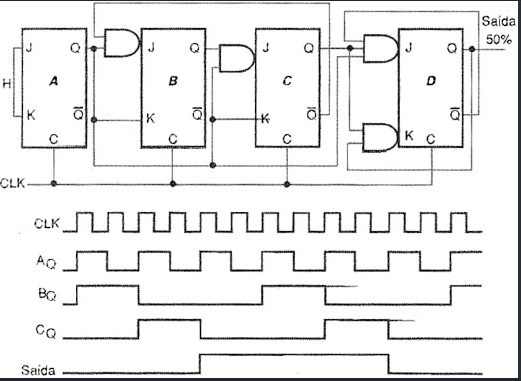
\includegraphics[
        width=\linewidth,
        height=0.65\textheight,
        keepaspectratio
    ]{images/divisor_de_frequencia.png}
    
\end{frame}